\documentclass{beamer}

% opacity bugfix: see http://tug.org/pipermail/pdftex/2007-December/007480.html
\pdfpageattr {/Group << /S /Transparency /I true /CS /DeviceRGB>>}

\usepackage[utf8]{inputenc}
\usepackage[OT1]{fontenc}

\usepackage{tikz}
\usetikzlibrary{%
   arrows,%
   calc,%
   fit,%
   patterns,%
   plotmarks,%
   shapes.geometric,%
   shapes.misc,%
   shapes.symbols,%
   shapes.arrows,%
   shapes.callouts,%
   shapes.multipart,%
   shapes.gates.logic.US,%
   shapes.gates.logic.IEC,%
   er,%
   automata,%
   backgrounds,%
   chains,%
   topaths,%
   trees,%
   petri,%
   mindmap,%
   matrix,%
   calendar,%
   folding,%
   fadings,%
   through,%
   patterns,%
   positioning,%
   scopes,%
   decorations.fractals,%
   decorations.shapes,%
   decorations.text,%
   decorations.pathmorphing,%
   decorations.pathreplacing,%
   decorations.footprints,%
   decorations.markings,%
   shadows}
\usepackage{animate}
\usepackage{amssymb, amsmath, amsfonts, enumerate}
\usepackage{pifont}
%\usepackage{bbold}
\newcommand\hmmax{0}
\usepackage{bm}
%\usepackage{dsfont}
\usepackage{pxfonts}
\usepackage{xcolor}
\usepackage{url}

\usepackage[backend=bibtex,style=authoryear,dashed=false]{biblatex}
\addbibresource{all.bib}
\addbibresource{lundrefs.bib}
\renewcommand{\bibfont}{\normalfont\scriptsize}
\setlength{\bibhang}{3ex}

\usepackage{hyperref}

\usetheme[official=false,department=none]{tue2008}
%\usefonttheme{default}


%\usetheme[secheader]{Boadilla}
%\setbeamercovered{transparent}
%\setbeamercovered{invisible}
%\setbeamertemplate{navigation symbols}{}
%\setbeamertemplate{bibliography item}[text] % numbered references
%\useoutertheme{infolines}
%\setbeamertemplate{headline}{}
%\setbeamertemplate{footline}{\hspace*{5mm}\hfill\insertframenumber\hspace*{5mm}\vspace{3mm}}
%\setbeamercolor{alerted text}{fg=orange!80!black}

% ------------------------------------------------------------------------------

\newcommand{\vcenterbox}[1]{\ensuremath{\vcenter{\hbox{#1}}}}
%
\newcommand{\reals}{\mathbb{R}}
\newcommand{\posreals}{\reals_{>0}}
\newcommand{\posrealszero}{\reals_{\ge 0}}
\newcommand{\naturals}{\mathbb{N}}

\newcommand{\dd}{\,\mathrm{d}}

\newcommand{\mbf}[1]{\mathbf{#1}}
\newcommand{\bs}[1]{\boldsymbol{#1}}
\renewcommand{\vec}[1]{{\bm#1}}

\newcommand{\uz}{^{(0)}} % upper zero
\newcommand{\un}{^{(n)}} % upper n
\newcommand{\ui}{^{(i)}} % upper i
\newcommand{\uell}{^{(\ell)}} % upper ell

\newcommand{\ul}[1]{\underline{#1}}
\newcommand{\ol}[1]{\overline{#1}}

\newcommand{\Tsys}{T_\text{sys}}
\newcommand{\fsys}{f_\text{sys}}

\newcommand{\Rsys}{R_\text{sys}}
\newcommand{\lRsys}{\ul{R}_\text{sys}}
\newcommand{\uRsys}{\ol{R}_\text{sys}}

\newcommand{\Fsys}{F_\text{sys}}
\newcommand{\lFsys}{\ul{F}_\text{sys}}
\newcommand{\uFsys}{\ol{F}_\text{sys}}


\def\tmax{t_\text{max}}
\def\tnow{t_\text{now}}
\def\tpnow{t^+_\text{now}}

\newcommand{\ptk}{p^k_t}

\def\yknow{y_k^{(\tnow)}}
\def\nknow{n_k^{(\tnow)}}

\newcommand{\nk}{n_k}
\newcommand{\nkp}{n_k'}
\newcommand{\yk}{y_k}
\newcommand{\ykp}{y_k'}

\newcommand{\Rsysnow}{R^{(t_\text{now})}_\text{sys}}
\newcommand{\Tsysnow}{T^{(t_\text{now})}_\text{sys}}
\newcommand{\tsysnow}{t^{(t_\text{now})}_\text{sys}}
\newcommand{\fsysnow}{f^{(t_\text{now})}_\text{sys}}
\def\eknow{e_k^{(\tnow)}}
\def\cknow{c_k^{(\tnow)}}
\def\vectknow{\vec{t}_k^{(\tnow)}}
\def\Phinow{\Phi^{(\tnow)}}
\newcommand{\gnow}{g^{(\tnow)}}
\newcommand{\tausnow}{\tau_*^{(\tnow)}}
\newcommand{\tsetup}{\tau_{\text{setup}}}

\newcommand{\E}{\operatorname{E}}
\newcommand{\V}{\operatorname{Var}}
\newcommand{\sd}{\operatorname{sd}}

\newcommand{\wei}{\operatorname{Wei}} % Weibull Distribution
\newcommand{\ig}{\operatorname{IG}}   % Inverse Gamma Distribution
\newcommand{\ber}{\operatorname{Bernoulli}} 
\newcommand{\bin}{\operatorname{Binomial}}
\newcommand{\be}{\operatorname{Beta}} 
\newcommand{\bebin}{\operatorname{Beta-binomial}}
\newcommand{\norm}{\operatorname{N}}

\def\then{{\structure{$\rule[0.35ex]{2ex}{0.5ex}\!\!\!\blacktriangleright$}}}
\def\play{{\structure{$\blacktriangleright$}}}
\def\gplus{{\structure{\rule[0.45ex]{1.4ex}{0.4ex}\hspace{-0.9ex}\rule[0.0ex]{0.4ex}{1.3ex}\hspace{0.5ex}}}}
\def\gminus{{\structure{\rule[0.45ex]{1.4ex}{0.4ex}}}}


\def\yz{y\uz}
\def\yn{y\un}
%\def\yi{y\ui}
\newcommand{\yfun}[1]{y^{({#1})}}
\newcommand{\yfunl}[1]{\ul{y}^{({#1})}}
\newcommand{\yfunu}[1]{\ol{y}^{({#1})}}

\def\ykt{y_{k,t}}

\def\ykz{y\uz_k}
\def\ykn{y\un_k}

\def\yktz{y\uz_{k,t}}
\def\yktn{y\un_{k,t}}

\def\yzl{\ul{y}\uz}
\def\yzu{\ol{y}\uz}
\def\ynl{\ul{y}\un}
\def\ynu{\ol{y}\un}
\def\yil{\ul{y}\ui}
\def\yiu{\ol{y}\ui}

\def\ykzl{\ul{y}\uz_k}
\def\ykzu{\ol{y}\uz_k}
\def\yknl{\ul{y}\un_k}
\def\yknu{\ol{y}\un_k}

\def\yktzl{\ul{y}\uz_{k,t}}
\def\yktzu{\ol{y}\uz_{k,t}}
\def\yktnl{\ul{y}\un_{k,t}}
\def\yktnu{\ol{y}\un_{k,t}}


\def\nz{n\uz}
\def\nn{n\un}
%\def\ni{n\ui}
\newcommand{\nfun}[1]{n^{({#1})}}
\newcommand{\nfunl}[1]{\ul{n}^{({#1})}}
\newcommand{\nfunu}[1]{\ol{n}^{({#1})}}

\def\nkz{n\uz_k}
\def\nkn{n\un_k}
\newcommand{\nkzfun}[1]{n\uz_{#1}}

\def\nkt{n_{k,t}}

\def\nktz{n\uz_{k,t}}
\def\nktn{n\un_{k,t}}


\def\nzl{\ul{n}\uz}
\def\nzu{\ol{n}\uz}
\def\nnl{\ul{n}\un}
\def\nnu{\ol{n}\un}
\def\nil{\ul{n}\ui}
\def\niu{\ol{n}\ui}

\def\nkzl{\ul{n}\uz_k}
\def\nkzu{\ol{n}\uz_k}
\def\nknl{\ul{n}\un_k}
\def\nknu{\ol{n}\un_k}

\def\nktzl{\ul{n}\uz_{k,t}}
\def\nktzu{\ol{n}\uz_{k,t}}
\def\nktnl{\ul{n}\un_{k,t}}
\def\nktnu{\ol{n}\un_{k,t}}

\def\taut{\tau(\vec{t})}
\def\taux{\tau(\vec{x})}
\def\ttau{\tilde{\tau}}
\def\ttaut{\ttau(\vec{t})}
\def\ttaux{\ttau(\vec{x})}

\def\MZ{\mathcal{M}\uz}
\def\MN{\mathcal{M}\un}

\def\MkZ{\mathcal{M}\uz_k}
\def\MkN{\mathcal{M}\un_k}

\def\MktZ{\mathcal{M}\uz_{k,t}}
\def\MktN{\mathcal{M}\un_{k,t}}

\def\PZ{\Pi\uz}
\def\PN{\Pi\un}

\def\PkZ{\Pi\uz_k}
\def\PkN{\Pi\un_k}
\newcommand{\PZi}[1]{\Pi\uz_{#1}}

\def\PktZ{\Pi\uz_{k,t}}
\def\PktN{\Pi\un_{k,t}}
\newcommand{\PtZi}[1]{\Pi\uz_{#1,t}}
\newcommand{\PkZi}[1]{\Pi\uz_{k,#1}}

\newcommand{\az}{\alpha\uz}
\newcommand{\an}{\alpha\un}
\newcommand{\bz}{\beta\uz}
\newcommand{\bn}{\beta\un}


\def\blau#1{{\color{tuegreen}#1}}
\def\rot#1{{\color{tuered}#1}}
\def\gruen#1{{\color{tueblue}#1}}

\def\yzr{\rot{\yz}}
\def\ynr{\rot{\yn}}
\def\byzr{\rot{\byz}}
\def\bynr{\rot{\byn}}
\def\yzor{\rot{y\uz_1}}
\def\yzjr{\rot{y\uz_j}}
\def\yzkr{\rot{y\uz_k}}
\def\yzlr{\rot{\yzl}}
\def\yzur{\rot{\yzu}}
\def\ynjr{\rot{y\un_j}}
\def\ynlr{\rot{\ynl}}
\def\ynur{\rot{\ynu}}
\def\yzjlr#1{\rot{\ul{y}\uz_#1}}
\def\yzjur#1{\rot{\ol{y}\uz_#1}}

\def\yktzr{\rot{\yktz}}
\def\yktnr{\rot{\yktn}}

\def\nzg{\gruen{\nz}}
\def\nng{\gruen{\nn}}
\def\nzlg{\gruen{\nzl}}
\def\nzug{\gruen{\nzu}}
\def\nnlg{\gruen{\nnl}}
\def\nnug{\gruen{\nnu}}
\def\nzjlg#1{\gruen{\ul{n}\uz_#1}}
\def\nzjug#1{\gruen{\ol{n}\uz_#1}}

\def\nktzg{\gruen{\nktz}}
\def\nktng{\gruen{\nktn}}

\def\psib{\blau{\psi}}
\def\bpsib{\blau{{b}(\psi)}}


% ------------ shading start
\newsavebox{\tempbox}
\newcommand\leftrightshading[3]{%
  \begin{tikzfadingfrompicture}[name=inputtext]
    \node [text=white] {#1};
  \end{tikzfadingfrompicture}
  \begin{lrbox}{\tempbox}%
    \begin{tikzpicture}
      \node [text=white,inner sep=0pt,outer sep=0pt] (textnode) {#1};
      \shade[path fading=inputtext,fit fading=false,left color=#2,right color=#3]
      (textnode.south west) rectangle (textnode.north east);
    \end{tikzpicture}%
  \end{lrbox}
  % Now we use the fading in another picture:
  \usebox\tempbox{}%
}
% ------------ shading end


%\def\PZc{\mathrm I\!\Pi\uz}
\def\PZc{\leftrightshading{$\mathrm I\!\Pi\uz$}{blue}{red}}
\def\PktZc{\leftrightshading{${\mathrm I\!\Pi_{k,t}\uz}$}{blue}{red}}
%\def\PNc{\PN}
\def\PNc{\leftrightshading{$\mathrm I\!\Pi\un$}{blue}{red}}



%%\def\blau#1{{\color{lmugreen2}#1}}
%\def\rot#1{{\color{red}#1}}
%\def\gruen#1{{\color{blue}#1}}

\newcommand{\x}{\vec{x}}

\def\tnow{t_\text{now}}
\def\tpnow{t^+_\text{now}}

\newcommand{\cmark}{{\color{tuegreen}\ding{51}}}
\newcommand{\xmark}{{\color{tuered}\ding{55}}}

\newcommand{\comp}[1]{\raisebox{-1mm}{\tikz{\node[%type1
rectangle,rounded corners=0mm,draw,fill=tuepmsgreen!70,thick,inner sep=0pt,minimum size=4mm]{#1};}}}

\newcommand{\cyansec}[1]{\textcolor{tuecyan}{\large\bf #1}}
\newcommand{\cyanalert}[1]{\textcolor{tuecyan}{#1}}
\newcommand{\bluesec}[1]{\textcolor{tueblue}{\large\bf #1}}
\newcommand{\bluealert}[1]{\textcolor{tueblue}{#1}}

\setbeamertemplate{itemize item}{\tiny\raise1.5pt\hbox{\color{tueblue}$\blacktriangleright$}}

% ------------------------------------------------------------------------------


\title{Nonparametric Bayesian System Reliability\\ using Sets of Priors}

\author{\ul{Gero Walter}\inst{1}, Louis Aslett\inst{2}, Frank Coolen\inst{3}}
\institute{ \inst{1} Eindhoven University of Technology, Eindhoven, NL\\ 
            \inst{2} University of Oxford, Oxford, UK\\
            \inst{3} Durham University, Durham, UK \\[2ex]
            \url{g.m.walter@tue.nl} \\[2ex]
            
\includegraphics[height=9mm]{logos/tuelogo} \quad 
            
\includegraphics[height=9mm]{logos/university_of_oxford} \quad
            
\includegraphics[height=9mm]{logos/logounidurham-large} \quad
            
\includegraphics[height=9mm]{logos/dinalog-hp} }
\date{Hannover 2016-12-08}

\begin{document}

\frame{
\titlepage
}

\addtocounter{framenumber}{-1} 

\begin{frame}{System Reliability}

\begin{columns}
\begin{column}{0.3\textwidth}
\begin{tikzpicture}
[type1/.style={rectangle,draw,fill=tuepmsgreen!70,very thick,inner sep=0pt,minimum size=6mm},
 type2/.style={rectangle,draw,fill=tuepmsgreen!70,very thick,inner sep=0pt,minimum size=6mm},
 type3/.style={rectangle,draw,fill=tuepmsgreen!70,very thick,inner sep=0pt,minimum size=6mm},
 cross/.style={cross out,draw=red,very thick,minimum width=7mm, minimum height=5mm},
 hv path/.style={thick, to path={-| (\tikztotarget)}},
 vh path/.style={thick, to path={|- (\tikztotarget)}}]
\begin{scope}[scale=0.75]
\node[type1] (T1-2) at ( 1.2, 1.1) {1};
\node[type1] (T1-3) at ( 1.2,-1.1) {1};
\node[type1] (T1-5) at ( 2.8, 1.1) {1};
\node[type1] (T1-6) at ( 2.8,-1.1) {1};
\node[type2] (T2)   at ( 2.0, 0)   {2};
\node[type3] (T3)   at ( 4.3, 0)   {3};
\coordinate (start) at (0  ,0);
\coordinate (end)   at (4.9,0);
\coordinate (bista) at (0.4,0);
\coordinate (biend) at (3.6,0);
\path (bista)     edge[hv path] (start)
                  edge[vh path] (T1-2.west)
                  edge[vh path] (T1-3.west)
      (T1-2.east) edge[hv path] (T2.north)
      (T1-3.east) edge[hv path] (T2.south)
      (T2.north)  edge[vh path] (T1-5.west)
      (T2.south)  edge[vh path] (T1-6.west)
      (biend)     edge[vh path] (T1-5.east)
                  edge[vh path] (T1-6.east)
                  edge[hv path] (T3.west)
      (T3.east)   edge[hv path] (end);
\end{scope}
\end{tikzpicture}
\end{column}
\begin{column}{0.7\textwidth}
We want to learn about the system reliability $\Rsys(t) = P(\Tsys > t)$ {\small (system survival function)}\\
based on
\begin{enumerate}
\item[\play]<2-> component test data:
 \begin{itemize}
 \item[] $n_k$ failure times for components of type $k$, $k = 1, \ldots, K$
 \end{itemize}
\item[\play]<3-> cautious assumptions\\ on component reliability:
 \begin{itemize}
 \item[] expert information,\\ e.g.\ from maintenance managers and staff
 \end{itemize}
\end{enumerate}
\end{column}
\end{columns}
\begin{center}
\uncover<4->{\cyanalert{How to combine these two information sources?}}
\end{center}
\end{frame}

\begin{frame}{Bayesian Inference}
\vspace*{-2ex}
\begin{align*}
\begin{array}{ccccl}
\uncover<1->{\text{expert info}        & + & \text{data}                & \to & \text{complete picture} \\[1.5ex]}
\uncover<2->{\text{prior distribution} & + & \text{sample distribution} & \to & \text{posterior distribution} \\[1.5ex]
 f(p) & \times & f(s \mid p) & \propto & f(p \mid s) \\
 & & & & \qquad\text{\bluealert{\play\ Bayes' Rule}} \\}
%\uncover<3->{\downarrow & & \downarrow & & \hspace*{3ex} \downarrow \\
\uncover<4->{\text{Beta prior}}   & & \uncover<3->{\text{Binomial}}         & & \uncover<5->{\text{Beta posterior}} \\
\uncover<4->{}                    & & \uncover<3->{\text{distribution}}     & & \uncover<5->{\qquad \text{\bluealert{\play\ conjugacy}}}\\[1ex]
\uncover<4->{p \sim \be(\az,\bz)} & & \uncover<3->{s \mid p \sim \bin(n,p)} & & \uncover<5->{p \mid s \sim \be(\an,\bn)}
\end{array}
\end{align*}
\vspace*{-3ex}
\begin{tikzpicture}
\uncover<6->{%
\node at (0,0) {\parbox{0.99\textwidth}{%
\begin{itemize}
\item conjugate prior makes learning about parameter tractable,\\  %posterior distribution
      just update hyperparameters:\quad $\az \to \an$, $\bz \to \bn$
\item closed form for many inferences, e.g. $\E[p\mid s] = \frac{\an}{\an+\bn}$
\end{itemize}}};}
\uncover<3-5>{%
\node at (-0.5,0) {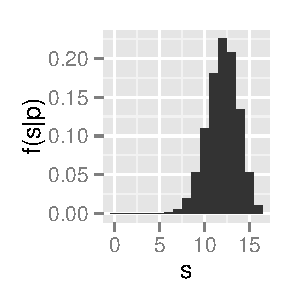
\includegraphics[width=0.25\textwidth]{figs/smallfig-binom}};}
\uncover<4-5>{%
\node at (-4.5,0) {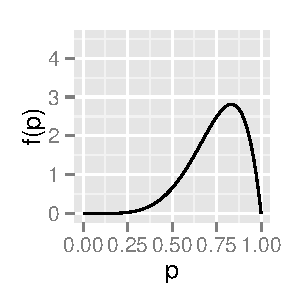
\includegraphics[width=0.25\textwidth]{figs/smallfig-prior}};}
\uncover<5>{%
\node at ( 3.5,0) {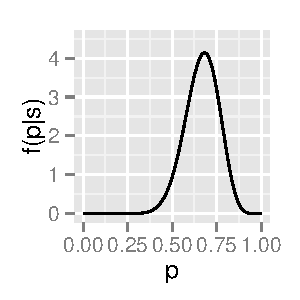
\includegraphics[width=0.25\textwidth]{figs/smallfig-posterior}};}
\end{tikzpicture}
\end{frame}

\begin{frame}{Nonparametric Component Reliability}
%nonparametric model for component failure time distribution\\
%example reliability curve on same frame?
\begin{tikzpicture}
\node at (1,3.5) %
{\parbox{\textwidth}{%
\uncover<1->{%
Functioning probability $\ptk$ of \comp{k} for each time $t \in {\cal T} = \{t'_1, t'_2, \ldots \}$\\
\quad\play\ discrete component reliability function $R^k(t) = p^k_t, \ t \in {\cal T}$.}}};
\uncover<2>{\node at (0,0) {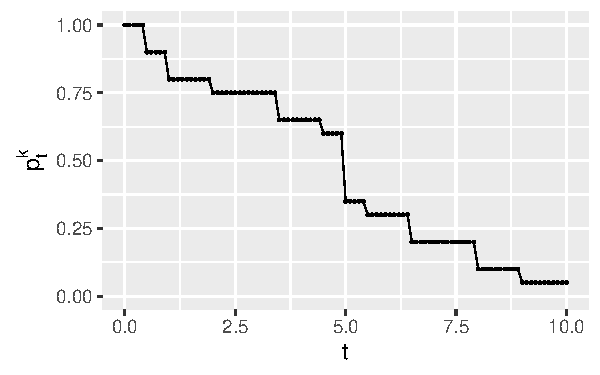
\includegraphics[width=0.7\textwidth]{figs/discr-rel-0.pdf}};}
\uncover<3>{\node at (0,0) {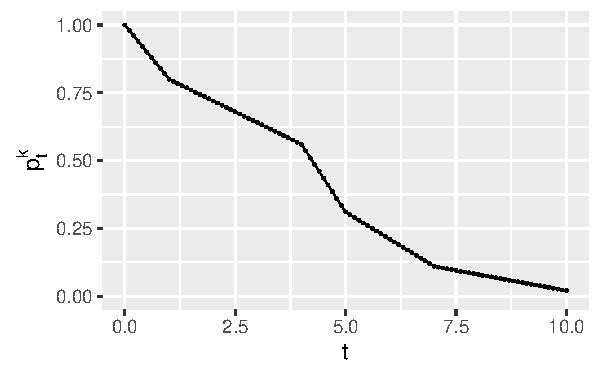
\includegraphics[width=0.7\textwidth]{figs/discr-rel-1.pdf}};}
\uncover<4>{\node at (0,0) {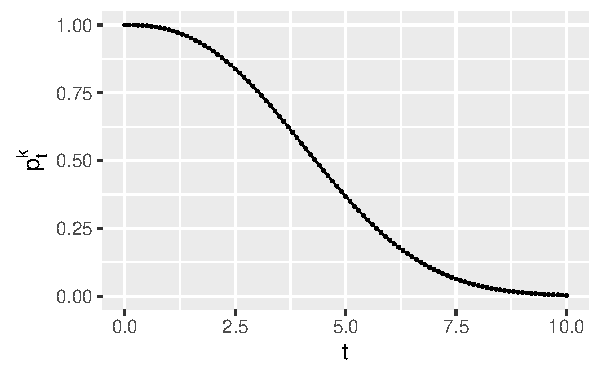
\includegraphics[width=0.7\textwidth]{figs/discr-rel-3.pdf}};}
\uncover<5>{\node at (0,0) {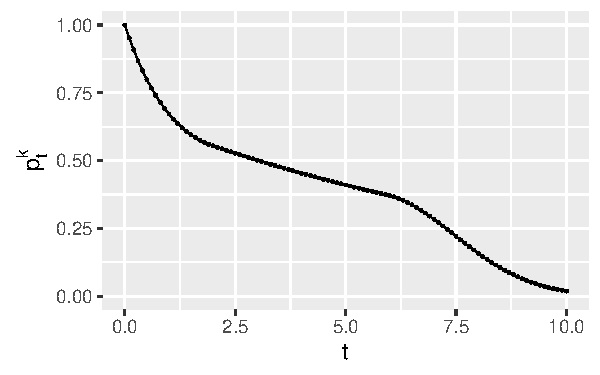
\includegraphics[width=0.7\textwidth]{figs/discr-rel-bt1.pdf}};}
\node at (1,0) %
{\parbox{\textwidth}{%
%\uncover<6->{%
%Choosing $\ptk$'s directly is hard (also ignores uncertainty in choice)\\}
\uncover<6->{%
\cyanalert{use Bayesian inference to estimate $\ptk$'s:}} %combine information from
\begin{itemize}
\item[\play]<7-> failure times $\vec{t}^k = (t^k_1, \ldots, t^k_{n_k})$ from component test data
 \begin{itemize}
 \item[] number of type $k$ components functioning at $t$:\\
 $S^k_t \mid \ptk \sim \bin(\ptk, n_k)$
 \end{itemize}
\item[\play]<8-> expert knowledge
 \begin{itemize}
 \item[] Beta prior for each $k$ and $t$:\\
 $\ptk \sim \be(\az_{k,t}, \bz_{k,t})$ %\hspace{6ex} \uncover<10->{$\nz_{k,t} = \az_{k,t} + \bz_{k,t}$,
                                       %                            \quad $\yz_{k,t} = \frac{\az_{k,t}}{\az_{k,t} + \bz_{k,t}} = \E[\ptk]$}
 \end{itemize}
\item[\play]<9-> complete picture
 \begin{itemize}
 \item[] Beta posterior for each $k$ and $t$:\\ %[1ex]
 $\ptk \mid s^k_t \sim \be(\an_{k,t}, \bn_{k,t})$ %\hspace{3ex} \uncover<12->{$\nn_{k,t} = \nz_{k,t} + n_k$} \\
%\hspace*{15ex} \uncover<12->{$\yn_{k,t} = \frac{\nz_{k,t}}{\nz_{k,t} + n_k} \, \yz_{k,t} + \frac{n_k}{\nz_{k,t} + n} \cdot \frac{s^k_t}{n_k}$}
 \end{itemize}
\end{itemize}}};
\end{tikzpicture}

\end{frame}

\begin{frame}{Prior-Data Conflict}

What if expert information and data tell different stories?\\
\begin{tikzpicture}
[pfeil/.style={-latex', line width=1mm, color=tuered, shorten <=1mm},
 cyanrand/.style={rounded corners, text centered, draw=tuecyan!50, inner sep=1mm, line width=0.7mm},
 redbrace/.style={draw=tuered, decoration=brace, decorate, line width=0.8mm},
 redbox/.style={text centered, draw=tuered, inner sep=1.5mm, line width=1mm, minimum width=0.75\textwidth}]
\uncover<2>{%
\node at (0,0) %
{\parbox{\textwidth}{%
\begin{block}{Prior-Data Conflict}
\begin{itemize}
\item \emph{informative prior beliefs} and \emph{trusted data}\\ %\rule{0ex}{3ex}\\
(sampling model correct, no outliers, etc.) are in conflict%\\%[2ex]
\item ``[\ldots] the prior [places] its mass primarily on distributions
in the sampling model for which the observed data is surprising''\\
\parencite{2006:evans}
\item there are not enough data to overrule the prior
\end{itemize}
\end{block}%
}};}
\uncover<3->{%
\node at (0,1.7) %
{\parbox{\textwidth}{%
\play\ reparametrisation helps to understand effect of prior-data conflict:
}};}
\uncover<4->{%
\node at (0,0.2) {\parbox[c]{\textwidth}{%
\begin{align*}
\nzg &= \az + \bz\,,
&
\yzr &= \frac{\az}{\az + \bz}\,, \quad \text{which are updated as}\\%[1.5ex]
\nng &= \nzg + n\,, 
&
\ynr &=  \frac{\nzg}{\nzg + n} \, \yzr + \frac{n}{\nzg + n} \cdot \frac{s}{n}
\end{align*}
}};}
\uncover<5->{%
\node[cyanrand] (yz) at (-0.9,-1.9) {$\yzr = \E[p]$};
\draw [pfeil] (yz.north east) to [out= 30,in=260] ( 0.9,-0.65);
\draw [pfeil] (yz.north west) to [out=130,in=240] (-1.7,0.4);}
\uncover<6->{%
\node[cyanrand] (yn) at ( 1.4,-1.9) {$\ynr = \E[p \mid s]$};
\draw [pfeil] (yn.north)      to [out=130,in=280] (-1.4,-0.65);}
\uncover<7->{%
\node[cyanrand] (ml) at ( 4.3,-1.9) {ML estimator $\hat{p}$};
\draw [pfeil] (ml.north)      to [out=100,in=330] (3.6,-0.65);}
\uncover<8->{%
\node[cyanrand] (nz) at (-4  ,-1.9) {$\nzg =$ pseudocounts};
\draw [pfeil] (nz.north)      to [out=90,in=270] (-4.0,-0.65);
\draw [pfeil] (nz.north west) to [out=95,in=240] (-5.2, 0.5);}
\uncover<9->{%
\node[redbox] at (0,-2.8) {$\E[p \mid s] = \ynr$ is a weighted average of $\E[p]$ and $\hat{p}$!};}
\uncover<10>{%
\node[redbox] at (0,-4.0) {$\V[p \mid s] = \dfrac{\ynr (1-\ynr)}{\nng + 1}$ decreases with $n$!};}
\end{tikzpicture}

\end{frame}

\begin{frame}{Sets of Priors}

%\item[\play] 
\textbf{Add \alert{imprecision} as new modelling dimension:\\
\alert{Sets of priors}\ldots}
\begin{tikzpicture}
\node at (0,0) %
{\parbox{\textwidth}{%
\begin{itemize}%[<+->]
% \begin{itemize}
 \item[] \ldots\ model uncertainty in probability statements %***show lottery A, B box
         % How is uncertainty about $\Rsys(t)$ expressed?
 \item<3->[] \ldots\ allow for partial or vague information on $\ptk$'s
         % Choosing all these Beta parameters is hard \ldots\\
 \item<4->[] \ldots\ highlight prior-data conflict.
         % see later
\end{itemize} %
\begin{itemize}
\item<5-> Separate uncertainty \emph{whithin the model} (reliability statements)\\
% ie what do we expect to see if components follow a Weibull(3.5,2) 
from uncertainty \emph{about the model} (which parameters).
\item<6-> Systematic sensitivity analysis / robust Bayesian approach
\item<7-> \textcite{2009:WalterAugustin}, \textcite{2013:diss-gw}:\\
vary $(\nzg, \yzr)$ in a set $\PZc = [\nzlg, \nzug] \times [\yzlr, \yzur]$\\
\quad\play\ easy elicitation, tractability \& prior-data conflict sensitivity
\item<8-> Bounds for inferences (point estimate, prediction, \ldots)\\
by min/max over $\PZc$ %or $\PNc$
\end{itemize}
}};
\uncover<2>{%
\node at (0,0.7) %
{\parbox{\textwidth}{%
\begin{block}{Uncertainty about probability statements}
\centerline{smaller sets $=$ more precise probability statements}
\vspace*{1ex}
\parbox[t]{0.45\textwidth}{\centering \textbf{Lottery A}\\
                          Number of winning tickets:\\
                          exactly known as 5 out of 100\\
                          \play\ $P(\text{win}) = 5/100$}
\qquad
\parbox[t]{0.45\textwidth}{\centering \textbf{Lottery B}\\
                          Number of winning tickets:\\
                          not exactly known, supposedly\\
                          between 1 and 7 out of 100\\
                          \play\ $P(\text{win}) = [1/100,\, 7/100]$}
\end{block} %
}};}
\end{tikzpicture}

%***or slide 9 from talk-lund???
%\uncover<7->{\quad\play\ min and max $\Rsys(t)$ over $\PZ$ analytical in most cases!}
%$\min_{\PZ} P\left(\Tsys > t \mid \{\nz_{k,t},\yz_{k,t},\vec{t}^k\}^{1:K}\right)$

\end{frame}

\begin{frame}{Component Reliability with Sets of Priors}

\begin{tikzpicture}
\uncover<1>{\node at (0,0) {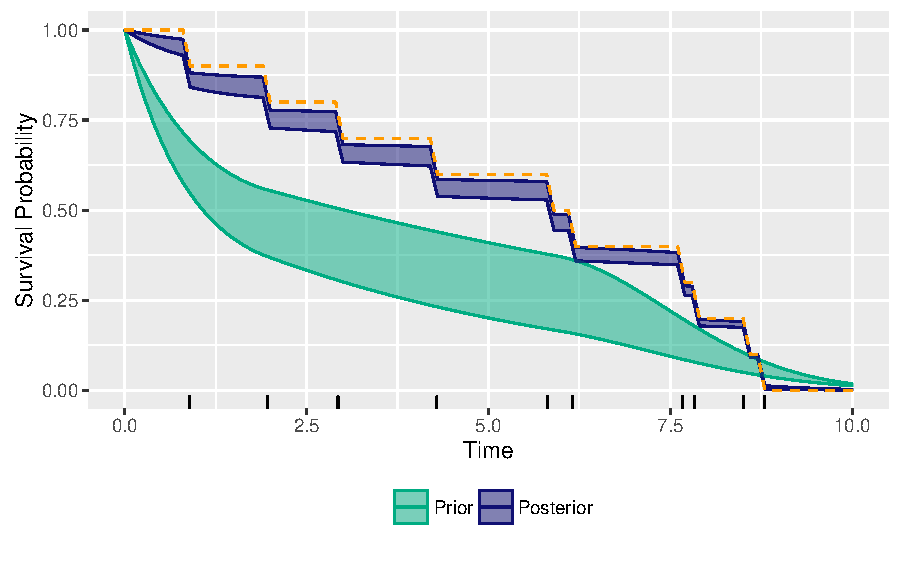
\includegraphics[width=\textwidth]{figs/T2p.pdf}};}
\uncover<1>{\node at (-3,-3.25) {\parbox{15ex}{$[\nzlg, \nzug] = [1,2]$\\ $[\yzlr, \yzur] = \ \updownarrow$}};}
\uncover<2>{\node at (0,0) {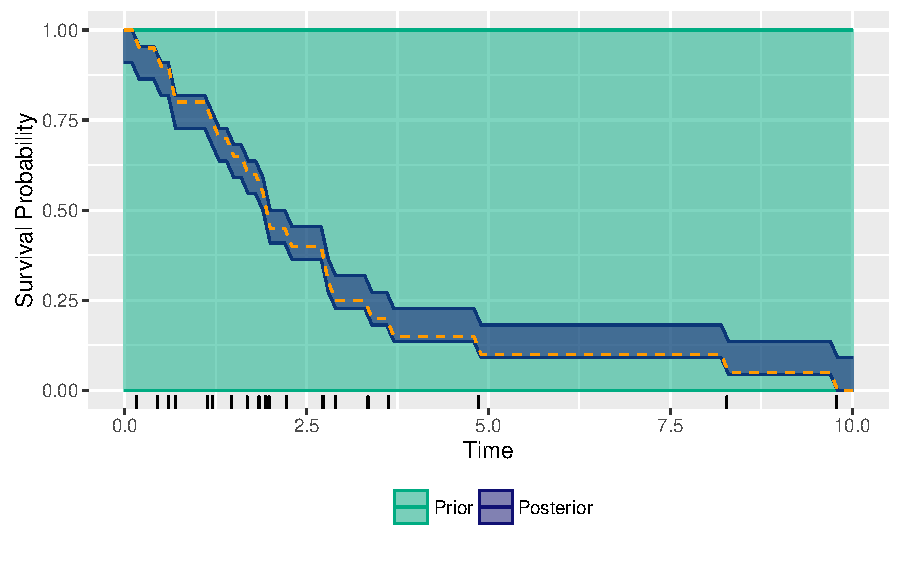
\includegraphics[width=\textwidth]{figs/T1p.pdf}};}
\uncover<2>{\node at (-3,-3.25) {\parbox{15ex}{$[\nzlg, \nzug] = [1,2]$\\ $[\yzlr, \yzur] = (0,1)$}};}
\uncover<3>{\node at (0,0) {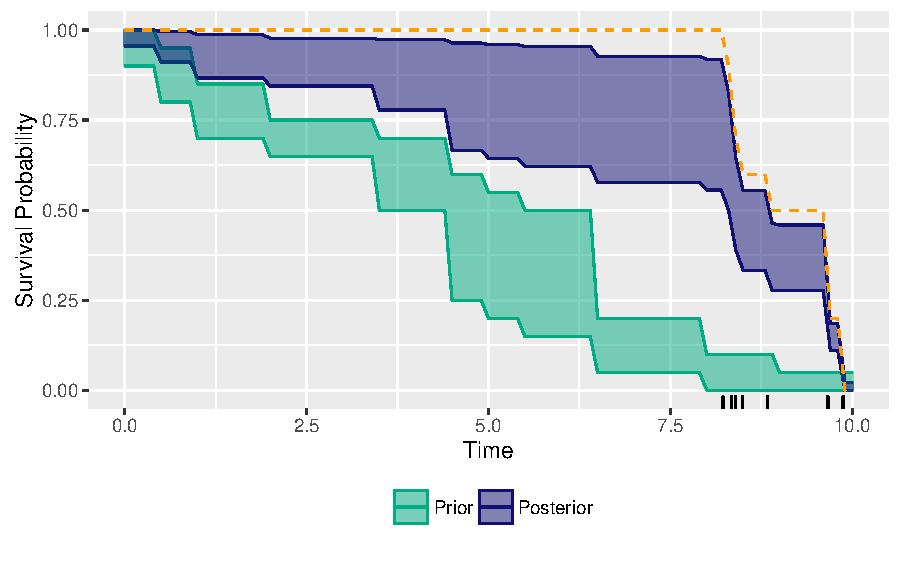
\includegraphics[width=\textwidth]{figs/T3p.pdf}};}
\uncover<3>{\node at (-3,-3.25) {\parbox{15ex}{$[\nzlg, \nzug] = [1,8]$\\ $[\yzlr, \yzur] = \ \updownarrow$}};}
\end{tikzpicture}

\end{frame}

\begin{frame}{System Reliability}

%(adapt slide 8 of ESREL talk)\\
%cite risk analysis paper\\
%frame with example graph?
\play\ Closed form for the system reliability via the survival signature:\\[-2ex]
\begin{tikzpicture} % l b r t
[cyanbox/.style={rounded corners, text centered, fill=tuecyan!20, inner sep=5mm},
 cyanrand/.style={rounded corners, text centered, draw=tuecyan!50, inner sep=2mm, very thick, font=\footnotesize},
 type1/.style={rectangle,draw,fill=tuepmsgreen!70,very thick,inner sep=0pt,minimum size=6mm},
 type2/.style={rectangle,draw,fill=tuepmsgreen!70,very thick,inner sep=0pt,minimum size=6mm},
 type3/.style={rectangle,draw,fill=tuepmsgreen!70,very thick,inner sep=0pt,minimum size=6mm},
 type1a/.style={rectangle,draw,fill=tueyellow!70,very thick,inner sep=0pt,minimum size=6mm},
 hv path/.style={thick, to path={-| (\tikztotarget)}},
 vh path/.style={thick, to path={|- (\tikztotarget)}},
 pfeil/.style={-latex', line width=1mm, color=tuered, shorten <=1mm}]
\uncover<1->{\node at (0,0) %
     {\parbox{\textwidth}{\begin{multline*}
       \Rsys\Big( t \mid {\textstyle \bigcup_{k=1}^K} \big\{\nktzg,\yktzr,\vec{t}^k\big\} \Big) = P(\Tsys > t \mid \cdots )\\
       = \sum_{l_1=0}^{m_1} \cdots \sum_{l_K=0}^{m_K} \Phi(l_1,\ldots,l_K)
         \prod_{k=1}^K P(C^k_t = l_k\mid\nktzg,\yktzr,\vec{t}^k)\end{multline*}}};}
\uncover<2->{\node[cyanrand] (survsign) at (-3.1,-3.6)%
     {\parbox[c]{0.51\textwidth}{Survival signature $\Phi(l_1,\ldots,l_K)$\\ \parencite{2012:survsign}\\
       $= P(\text{system functions} \mid \{l_k \text{ \comp{k}'s function}\}^{1:K})$\\[1ex]
      \begin{tabular}{ccc|l}
      $l_1$ & $l_2$ & $l_3$ & $\Phi$ \\
      \hline
      0 & 0 & 1 & 0 \\
      1 & 0 & 1 & 0 \\
      2 & 0 & 1 & 1/3 \\
      3 & 0 & 1 & 1 \\
      4 & 0 & 1 & 1 %\rule[-2.2ex]{0ex}{1ex}%\phantom{\vdots}
      \end{tabular} \hspace{1ex}
      \begin{tabular}{ccc|l}
      $l_1$ & $l_2$ & $l_3$ & $\Phi$ \\
      \hline
      0 & 1 & 1 & 0 \\
      1 & 1 & 1 & 0 \\
      2 & 1 & 1 & 2/3 \\
      3 & 1 & 1 & 1 \\
      4 & 1 & 1 & 1 
%      \vdots & \vdots & \vdots & \vdots
      \end{tabular} } };
\draw [pfeil] (survsign.north) to [out=50,in=260] (0.3,-0.7);}
\uncover<2-8>{%
\begin{scope}[xshift=1cm,yshift=-3.5cm]
\uncover<3-8>{\node at (0.5,1.7) {\cmark};}
\uncover<4-8>{\node at (1.0,1.7) {\cmark};}
\uncover<5-8>{\node at (1.5,1.7) {\xmark};}
\uncover<6-8>{\node at (2.0,1.7) {\xmark};}
\uncover<7-8>{\node at (2.5,1.7) {\xmark};}
\uncover<8-8>{\node at (3.0,1.7) {\xmark};}
\begin{scope}[scale=0.75]
\uncover<2,4,6,8>{\node[type1 ] (T1-2) at ( 1.2, 1.1) {1};}
\uncover<3,5,7>  {\node[type1a] (T1-2) at ( 1.2, 1.1) {1};}
\uncover<2,3,6,7>{\node[type1 ] (T1-3) at ( 1.2,-1.1) {1};}
\uncover<4,5,8>  {\node[type1a] (T1-3) at ( 1.2,-1.1) {1};}
\uncover<2,4,5,7>{\node[type1 ] (T1-5) at ( 2.8, 1.1) {1};}
\uncover<3,6,8>  {\node[type1a] (T1-5) at ( 2.8, 1.1) {1};}
\uncover<2,3,5,8>{\node[type1 ] (T1-6) at ( 2.8,-1.1) {1};}
\uncover<4,6,7>  {\node[type1a] (T1-6) at ( 2.8,-1.1) {1};}
\node[type2] (T2)   at ( 2.0, 0)   {2};
\node[type3] (T3)   at ( 4.3, 0)   {3};
\coordinate (start) at (0  ,0);
\coordinate (end)   at (4.9,0);
\coordinate (bista) at (0.4,0);
\coordinate (biend) at (3.6,0);
\path (bista)     edge[hv path] (start)
                  edge[vh path] (T1-2.west)
                  edge[vh path] (T1-3.west)
      (T1-2.east) edge[hv path] (T2.north)
      (T1-3.east) edge[hv path] (T2.south)
      (T2.north)  edge[vh path] (T1-5.west)
      (T2.south)  edge[vh path] (T1-6.west)
      (biend)     edge[vh path] (T1-5.east)
                  edge[vh path] (T1-6.east)
                  edge[hv path] (T3.west)
      (T3.east)   edge[hv path] (end);
\end{scope}
\end{scope}}
\uncover<9>{\node[cyanrand] (postpred) at (3,-3.6)%
     {\parbox[c]{0.41\textwidth}{Posterior predictive probability that\\ in a new system, $l_k$ of the $m_k$ \comp{k}'s\\
                                function at time $t$:\\[1ex] \hspace*{1ex}
                                $\binom{m_k}{l_k} \int [P(T_k >   t \mid \ptk)]^{l_k}$ \\ \hspace*{5.6ex}
                                                      $[P(T_k \le t \mid \ptk)]^{m_k-l_k}$ \\ \hspace*{6ex}
%                                $f(\ptk \mid \az_{k,t},\bz_{k,t},\vec{t}^k)\, d\ptk $\\[1ex] \hspace*{5ex}
%                                $= \binom{m_k}{l_k} \frac{B(      \az_{k,t} + s^k_t,             \bz_{k,t} + n_k - s^k_t)}%
%                                                         {B(l_k + \az_{k,t} + s^k_t, m_k - l_k + \bz_{k,t} + n_k - s^k_t)}$}};
                                $f(\ptk \mid \nktzg,\yktzr,\vec{t}^k)\, d\ptk $\\[1ex] %\hspace*{5ex}
\play\ analytical solution for integral:\\
\hspace*{2ex}$C^k_t \mid \nktzg,\yktzr,\vec{t}^k \sim \bebin$}};
\draw [pfeil] (postpred.north) to [out=90,in=270] (3.0,-0.7);}
\end{tikzpicture}

\end{frame}

\begin{frame}{System Reliability Bounds}

\play\ Bounds for $\Rsys\Big(\,t\,\big|\, \bigcup\limits_{k=1}^K \Big\{\nktzg,\yktzr,\vec{t}^k\Big\}\Big)$
over $\bigcup\limits_{k=1}^K \Big\{$\raisebox{-1.05ex}{$\PktZc$}$\Big\}$:
\begin{itemize}[<+->]
\item $\min \Rsys(\cdot)$ by $\yktzr = \yzjlr{{k,t}}$ for any $\nktzg$\\
%(first-order stochastic dominance of posterior predictive along $\yktzr$)
\parencite[Theorem 1]{2017:walter-aslett-coolen}
\item $\min \Rsys(\cdot)$ for $\nzjlg{{k,t}}$ or $\nzjug{{k,t}}$ according to simple conditions\\
%conditions on $\yzjlr{{k,t}}$
\parencite[Theorem 2 \& Lemma 3]{2017:walter-aslett-coolen}
\item numeric optimization over $[\nzjlg{{k,t}}, \nzjug{{k,t}}]$
in the very few cases\\ where Theorem 2 \& Lemma 3 do not apply
\item implemented in \textbf{R} package \texttt{ReliabilityTheory} \parencite{2016:aslett-RT}
\end{itemize}
%so analytical in most cases!

\end{frame}


\begin{frame}{System Reliability Bounds}
\begin{tikzpicture}
[typeM/.style={rectangle,draw,fill=tuepmsgreen!70,thick,inner sep=0pt,minimum size=5mm,font=\footnotesize},
 typeC/.style={rectangle,draw,fill=tuepmsgreen!70,thick,inner sep=0pt,minimum size=5mm,font=\footnotesize},
 typeP/.style={rectangle,draw,fill=tuepmsgreen!70,thick,inner sep=0pt,minimum size=5mm,font=\footnotesize},
 typeH/.style={rectangle,draw,fill=tuepmsgreen!70,thick,inner sep=0pt,minimum size=5mm,font=\footnotesize},
 cross/.style={cross out,draw=red,very thick,minimum width=7mm, minimum height=5mm},
 hv path/.style={thick, to path={-| (\tikztotarget)}},
 vh path/.style={thick, to path={|- (\tikztotarget)}}]
\node at (0,0) {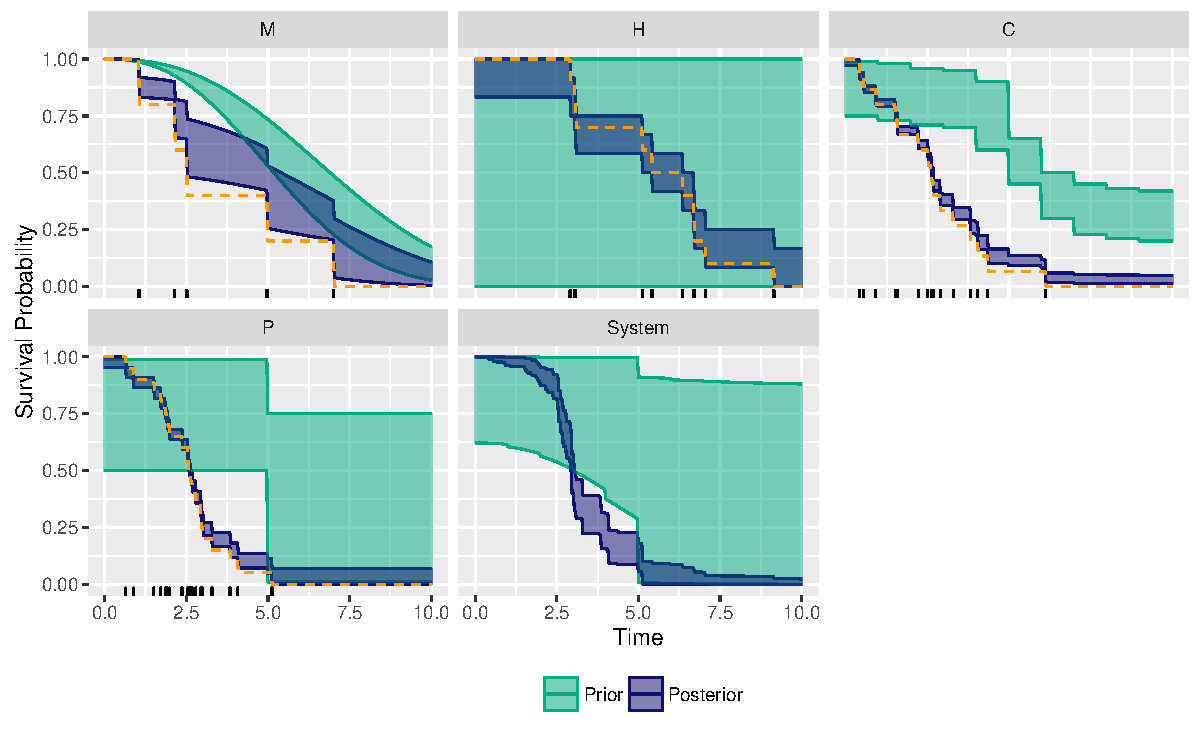
\includegraphics[width=\textwidth]{figs/brakingsystem-dagstat16.pdf}};
\begin{scope}[scale=0.90,xshift=3.4cm,yshift=-1.1cm]
\node[typeM] (M)    at ( 0  , 0  ) {M};
\node[typeC] (C1)   at ( 1  , 1.5) {C1};
\node[typeC] (C2)   at ( 1  , 0.5) {C2};
\node[typeC] (C3)   at ( 1  ,-0.5) {C3};
\node[typeC] (C4)   at ( 1  ,-1.5) {C4};
\node[typeP] (P1)   at ( 2  , 1.5) {P1};
\node[typeP] (P2)   at ( 2  , 0.5) {P2};
\node[typeP] (P3)   at ( 2  ,-0.5) {P3};
\node[typeP] (P4)   at ( 2  ,-1.5) {P4};
\node[typeH] (H)    at ( 0  ,-1  ) {H};
\coordinate (start)  at (-0.7, 0);
\coordinate (startC) at ( 0.5, 0);
\coordinate (startH) at (-0.4, 0);
\coordinate (Hhop1)  at ( 0.4,-1);
\coordinate (Hhop2)  at ( 0.6,-1);
\coordinate (endP)   at ( 2.5, 0);
\coordinate (end)    at ( 2.8, 0);
\path (start)     edge[hv path] (M.west)
      (M.east)    edge[hv path] (startC)
      (startC)    edge[vh path] (C1.west)
                  edge[vh path] (C2.west)
                  edge[vh path] (C3.west)
                  edge[vh path] (C4.west)
      (C1.east)   edge[hv path] (P1.west)
      (C2.east)   edge[hv path] (P2.west)
      (C3.east)   edge[hv path] (P3.west)
      (C4.east)   edge[hv path] (P4.west)
      (endP)      edge[vh path] (P1.east)
                  edge[vh path] (P2.east)
                  edge[vh path] (P3.east)
                  edge[vh path] (P4.east)
                  edge[hv path] (end)
      (startH)    edge[vh path] (H.west)
      (H.east)    edge[hv path] (Hhop1)
      (Hhop1)     edge[thick,out=90,in=90] (Hhop2)
      (Hhop2)     edge[hv path] (P3.south)
                  edge[hv path] (P4.north);
\end{scope}
\end{tikzpicture}
\end{frame}

\begin{frame}{Summary \& Outlook}

%(adapt slide 11 of ESREL talk)\\
%case study\\
%block policy with minimal repair?\\
%(nonparam hazard rate $h^k(t_j) = (p^k_{t_j} - p^k_{t_{j+1}}) / p^k_{t_j}$)
\uncover<1->{%
\textbf{Summary:}
\begin{itemize}
\item[\play] Nonparametric modeling of component reliability curves
\item[\play] Bayesian model combining expert knowledge and test data
\item[\play] Set of system reliability functions %appropriately
reflects uncertainties from limited data, vague expert information, and prior-data conflict
\item[\play] Easy-to-use implementation in \textbf{R} package \texttt{ReliabilityTheory} \parencite{2016:aslett-RT}
\end{itemize}}
\uncover<2->{%
\textbf{Next steps:}
\begin{itemize}
\item[\play] Allow right-censored observations (RUL estimation)
\item[\play] Allow dependence between components\\ (common-cause failure, \ldots) %or more explicit dependence
\item[\play] Use for system design (where to put extra redundancy?)
\item[\play] Use for maintenance planning
\end{itemize}}
\end{frame}


\title{Condition-Based Maintenance Policies\\ for Complex Systems\\ using Component Status Montoring}

\author{Gero Walter, Simme Douwe Flapper}
\institute{Eindhoven University of Technology, Eindhoven, NL\\ 
           \url{g.m.walter@tue.nl} \\[2ex]
           
\includegraphics[height=9mm]{logos/tuelogo} \quad 
           
\includegraphics[height=9mm]{logos/dinalog-hp} }
\date{Hannover 2016-12-08}

\frame{
\titlepage
}

%\addtocounter{framenumber}{-1}

\begin{frame}{\large Dynamic \& Adaptive Residual Life Distributions}
\begin{tikzpicture}
[typeA/.style={rectangle,draw,fill=tuepmsgreen!70,very thick,inner sep=0pt,minimum size=6mm},
 typeB/.style={rectangle,draw,fill=tueyellow!50,very thick,inner sep=0pt,minimum size=6mm},
 cross/.style={cross out,draw=red,very thick,minimum width=7mm, minimum height=5mm},
 hv path/.style={very thick, to path={-| (\tikztotarget)}},
 vh path/.style={very thick, to path={|- (\tikztotarget)}},
 comparrow/.style={draw,-stealth,tuered,line width=1mm},
 ellistyle/.style={draw,tuered,line width=0.5mm}]
\begin{scope}[scale=0.75]
\uncover<1->{%
\node[typeA] (A1) at ( 0, 1.2) {A};
\node[typeA] (A2) at ( 0, 0  ) {A};
%\uncover<2->{\node[cross] at (0,0) {};}
\node[typeB] (B1) at ( 0,-1.2) {B};
\coordinate (start) at (-1  ,0);
\coordinate (end)   at ( 1  ,0);
\coordinate (fork1) at (-0.7,0);
\coordinate (fork2) at ( 0.7,0);
\path (fork1) edge[vh path] (start)
              edge[vh path] (A1)
              edge[vh path] (A2)
              edge[vh path] (B1);
\path (fork2) edge[vh path] (end)
              edge[vh path] (A1)
              edge[vh path] (A2)
              edge[vh path] (B1);}
\uncover<2->{%
\node (compArel0) at (-3.5, 1.7) {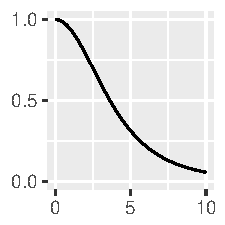
\includegraphics[width=2cm]{figs/compArel0}};
\node (compBrel0) at (-3.5,-1  ) {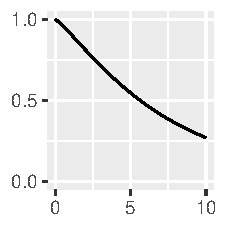
\includegraphics[width=2cm]{figs/compBrel0}};
%\path (compArel0.east) edge[comparrow, bend right] ($(A1.west) + (-0.5,0   )$)
%                       edge[comparrow, bend right] ($(A2.west) + (-0.5,0.25)$);
\draw [comparrow]   (compArel0.east)              to [out=-10,in=170] ($(A1.west) + (-0.2, 0.25)$);
\draw [comparrow] ($(compArel0.east) + (0,-0.2)$) to [out=-10,in=160] ($(A2.west) + (-0.4, 0.35)$);
\draw [comparrow]   (compBrel0.east)              to [out=-10,in=190] ($(B1.west) + (-0.2,-0.25)$);}
\uncover<3->{%
\draw [ellistyle] (0,0) ellipse (1.3 and 2.1);}
\end{scope}
\begin{scope}[xshift=5cm,scale=0.75]
\uncover<5->{%
\node[typeA] (A1) at ( 0, 1.2) {A};
%\node[typeA] (A2) at ( 0, 0  ) {A};
%\uncover<2->{\node[cross] at (0,0) {};}
\node[typeB] (B1) at ( 0,-1.2) {B};
\coordinate (start) at (-1  ,0);
\coordinate (end)   at ( 1  ,0);
\coordinate (fork1) at (-0.7,0);
\coordinate (fork2) at ( 0.7,0);
\path (fork1) edge[vh path] (start)
              edge[vh path] (A1)
%             edge[vh path] (A2)
              edge[vh path] (B1);
\path (fork2) edge[vh path] (end)
              edge[vh path] (A1)
%              edge[vh path] (A2)
              edge[vh path] (B1);}
\uncover<6->{%
\node (compArel5) at (-3.5, 1.7) {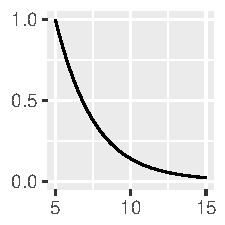
\includegraphics[width=2cm]{figs/compArel5}};
\node (compBrel5) at (-3.5,-1  ) {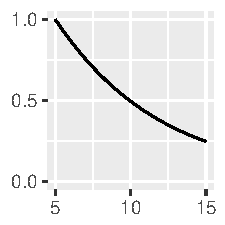
\includegraphics[width=2cm]{figs/compBrel5}};
\draw [comparrow]   (compArel5.east)              to [out=-10,in=170] ($(A1.west) + (-0.2, 0.25)$);
\draw [comparrow]   (compBrel5.east)              to [out=-10,in=190] ($(B1.west) + (-0.2,-0.25)$);}
\uncover<9->{%
\draw [ellistyle] (0,0) ellipse (1.3 and 2.1);}
\end{scope}
\begin{scope}[yshift=-2cm]
\uncover<4->{%
\draw[very thick, -stealth] (-1,0) -- (6,0);
\foreach \t in {0,5} \draw[very thick] (\t,0.1) -- (\t,-0.1) node[below] {\t};}
\uncover<3->{%
\node (sysABrel0) at (1, -1.7) {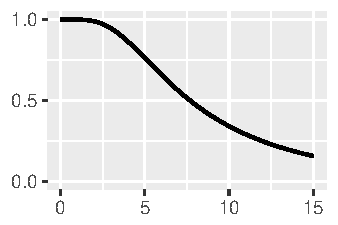
\includegraphics[width=3cm]{figs/sysABrel0}};
\draw [comparrow] (0.5,0.5) to [out=-45,in=90] ($(sysABrel0.north) + (0,-0.1)$);}
\uncover<9->{%
\node (sysABrel5) at (6, -1.7) {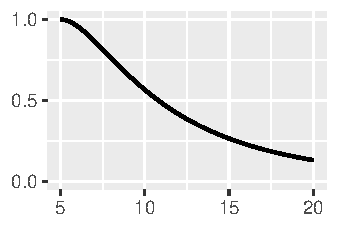
\includegraphics[width=3cm]{figs/sysABrel5}};
\draw [comparrow] (5.5,0.5) to [out=-45,in=90] ($(sysABrel5.north) + (0,-0.1)$);}
\end{scope}
\begin{scope}[xshift=7cm,yshift=-1cm]
\node at (0,0) {\parbox{0.23\textwidth}{%
\begin{itemize}
\item<7-> component ageing
\item<8-> model update
\item<10-> system layout
\end{itemize}
}};
\end{scope}
\end{tikzpicture}
\end{frame}

\begin{frame}{\large Dynamic \& Adaptive Maintenance Policy}
\begin{tikzpicture}
\uncover<1-3>{%
\node (sysABrelhist) at (-0.79, 0) {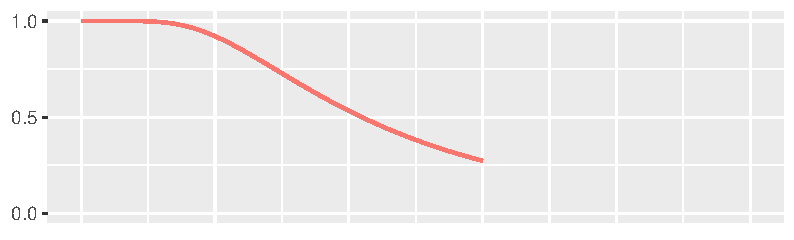
\includegraphics[width=0.865\textwidth]{figs/sysABrelhist1}};}
\uncover<2-3>{%
\node (sysABrelhist) at ( 0   ,-3) {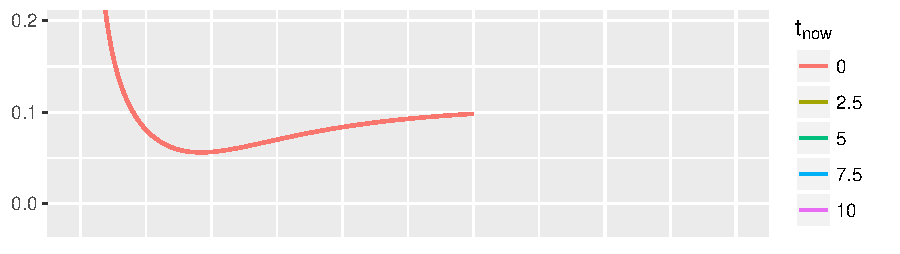
\includegraphics[width=     \textwidth]{figs/sysABghist1}};}
\uncover<3>{%
\node (sysABtau)     at (-0.59,-5) {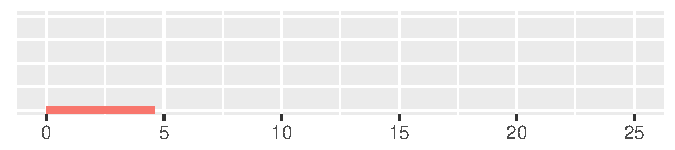
\includegraphics[width=0.838\textwidth]{figs/sysABtau1}};
%\draw[dotted, very thick] (-3.75,-3.75) -- (-3.75,-5.45);}
\draw[dotted, very thick] (-3.275,-3.35) -- (-3.275,-5.45);}
\uncover<4>{%
\node (sysABrelhist) at (-0.79, 0) {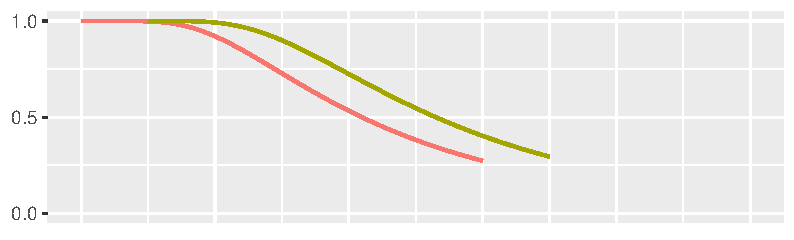
\includegraphics[width=0.865\textwidth]{figs/sysABrelhist2}};
\node (sysABrelhist) at ( 0   ,-3) {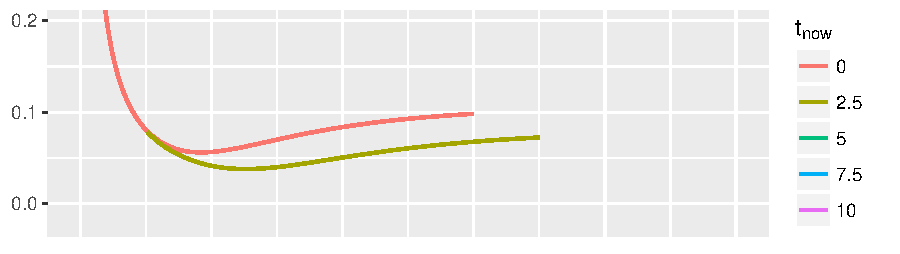
\includegraphics[width=     \textwidth]{figs/sysABghist2}};
\node (sysABtau)     at (-0.59,-5) {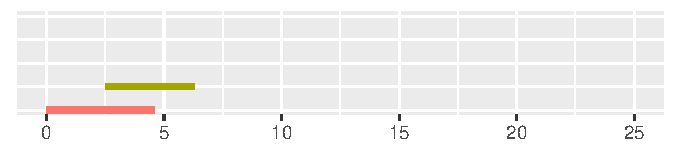
\includegraphics[width=0.838\textwidth]{figs/sysABtau2}};}
\uncover<5>{%
\node (sysABrelhist) at (-0.79, 0) {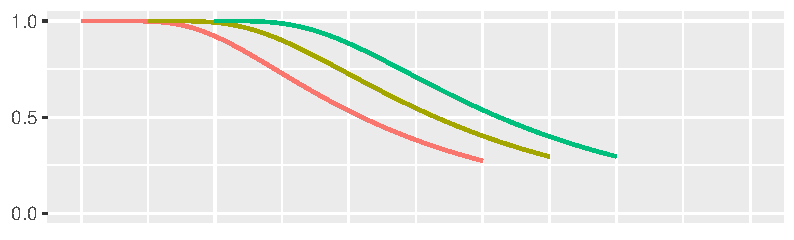
\includegraphics[width=0.865\textwidth]{figs/sysABrelhist3}};
\node (sysABrelhist) at ( 0   ,-3) {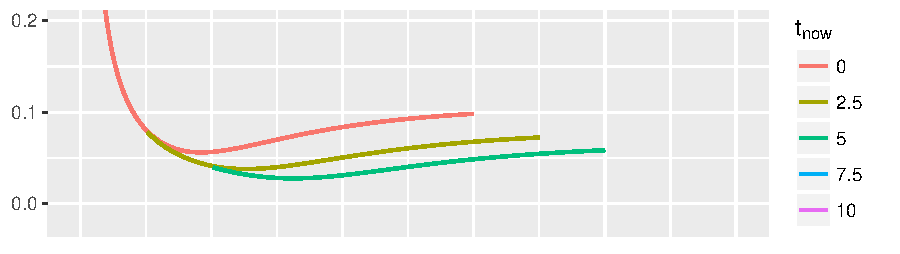
\includegraphics[width=     \textwidth]{figs/sysABghist3}};
\node (sysABtau)     at (-0.59,-5) {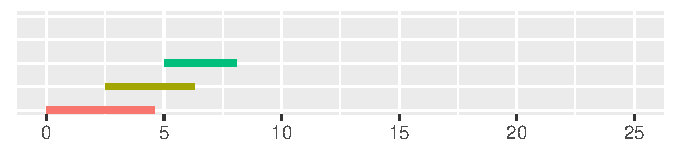
\includegraphics[width=0.838\textwidth]{figs/sysABtau3}};}
\uncover<6>{%
\node (sysABrelhist) at (-0.79, 0) {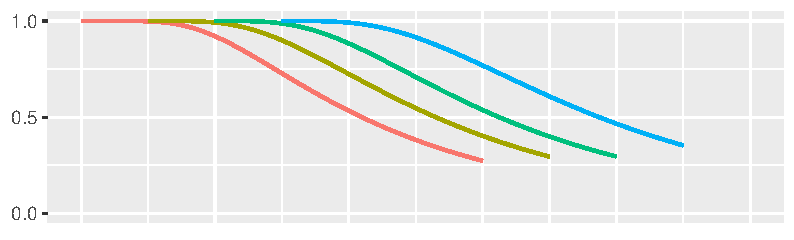
\includegraphics[width=0.865\textwidth]{figs/sysABrelhist4}};
\node (sysABrelhist) at ( 0   ,-3) {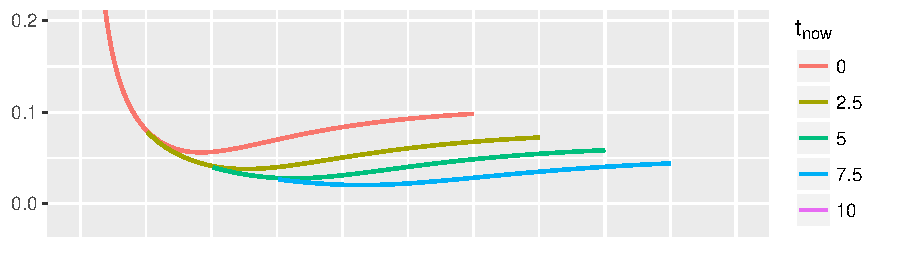
\includegraphics[width=     \textwidth]{figs/sysABghist4}};
\node (sysABtau)     at (-0.59,-5) {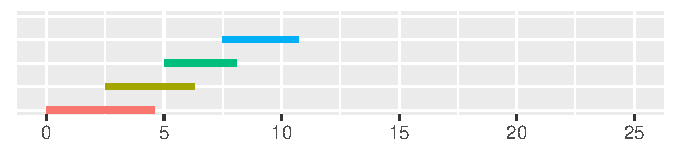
\includegraphics[width=0.838\textwidth]{figs/sysABtau4}};}
\uncover<7->{%
\node (sysABrelhist) at (-0.79, 0) {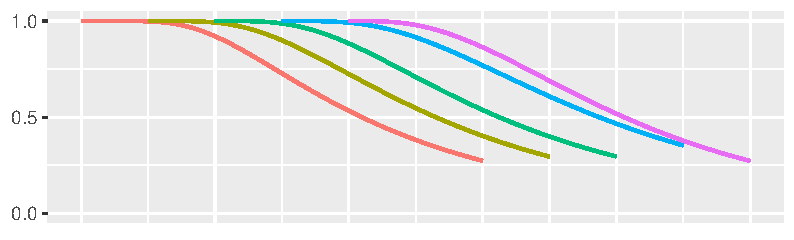
\includegraphics[width=0.865\textwidth]{figs/sysABrelhist5}};
\node (sysABrelhist) at ( 0   ,-3) {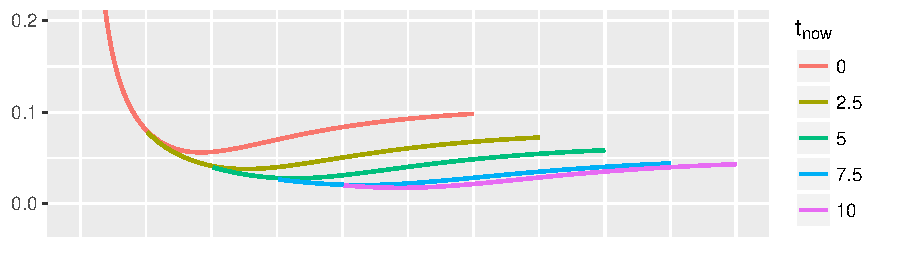
\includegraphics[width=     \textwidth]{figs/sysABghist5}};}
\uncover<7>{
\node (sysABtau)     at (-0.59,-5) {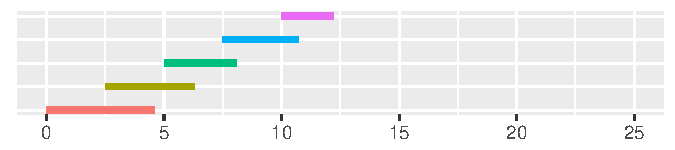
\includegraphics[width=0.838\textwidth]{figs/sysABtau5}};}
\uncover<8->{%
\node (sysABtau)     at (-0.59,-5) {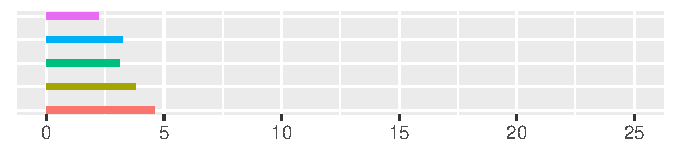
\includegraphics[width=0.838\textwidth]{figs/sysABtau5a}};}
\uncover<1->{%
\node[rotate=90] at (-6.1,0) {reliability};}
\uncover<2->{%
\node[rotate=90] at (-6.1,-2.5) {cost rate};}
\uncover<3->{%
\node[rotate=90] at (-6.1,-4.8) {\parbox{7ex}{\centering\scriptsize time to\\ maintenance}};}
\uncover<9>{%
\draw[<->, very thick] (-4.83,-6.2) -- (-4.0,-6.2) node[right] {time to next evaluation};
\draw[dashed, thick] (-4.0,-6.1) -- (-4.0,-4);}
\end{tikzpicture}
\end{frame}

\begin{frame}{\large System Reliability using the Survival Signature}
\begin{tikzpicture}
[cyanbox/.style={rounded corners, text centered, fill=tuecyan!20, inner sep=5mm},
 cyanrand/.style={rounded corners, text centered, draw=tuecyan!50, inner sep=2mm, very thick, font=\footnotesize},
 pfeil/.style={-latex', line width=1mm, color=tuered, shorten <=1mm}]
\node at (1,0) {\parbox{\textwidth}{%
\begin{itemize}
\item[$\Tsysnow$] (random) time of system failure given all info.\ at time $\tnow$
\item[$\Rsysnow(t)$] corresponding reliability function 
\item[$\cknow$] number of type $k$ components functioning at time $\tnow$
%\item[$\Phinow$] survival signature at $\tnow$\\
%$= P(\text{system functions} \mid \{l_k \text{ \comp{k}'s function}\}^{1:K})$
\item[$K$] number of component types
\end{itemize}}};
\node at (0,-2.5) {\parbox{\textwidth}{%
\begin{align*}
\Rsysnow(t) &= \sum_{l_1=0}^{c_1^{(\tnow)}} \cdots \sum_{l_K=0}^{c_K^{(\tnow)}} \Phinow(l_1,\ldots,l_K)
               \prod_{k=1}^K P(C^k_t = l_k\mid\nkz,\ykz, \vectknow)
\end{align*}}};
\uncover<2->{%
\draw[decorate,decoration=brace,line width=0.6mm] (0.75,-3.1)  -- (-1.7,-3.1) node[cyanrand, below=0.5cm] {\parbox{0.51\textwidth}{\centering%
survival signature at time $\tnow$\\
$= P(\text{system functions} \mid \{l_k \text{ \comp{k}'s function}\}^{1:K})$
}};}
\uncover<3->{%
\draw[decorate,decoration=brace,line width=0.6mm] (5.7,-3.1)  -- (1.6,-3.1) node[cyanrand, midway, below=0.5cm] {\parbox{0.3\textwidth}{%
Probability that $l_k$ of the $\cknow$ \comp{k}'s function
}};}
\end{tikzpicture}
\end{frame}

\begin{frame}{\large Expected Operational Cyle Cost Rate}
\hspace*{5ex}%
\begin{minipage}{0.8\textwidth}
\vspace*{3ex}%
\begin{itemize}
\item[$\tau$] decision variable (when to do maintenance?)
\item[$\Tsysnow$] (random) time of system failure,\\ with density \structure{$\fsysnow(t)$} and reliability function \structure{$\Rsysnow(t)$}
\item[$c_p$] cost of preventive maintenance action
\item[$c_c$] cost of corrective maintenance action
\end{itemize}
\end{minipage}
\begin{align*}
g(\tau \mid \Tsysnow = \tnow + t) =
\begin{cases}
c_c / (\tnow + t   )  & \text{if } t <   \tau \quad\text{(failure before $\tau$)} \\
c_p / (\tnow + \tau)  & \text{if } t \ge \tau \quad\text{(failure after $\tau$)}
\end{cases}
\end{align*}
\vspace*{-2ex}
\begin{align*}
\uncover<2->{%
\gnow(\tau) &= \E\Big[g(\tau \mid \Tsysnow)\Big] \\
            &= \frac{c_p}{\tnow + \tau} \Rsysnow(\tnow + \tau) + c_c \int_0^\tau \frac{1}{\tnow + t} \fsysnow(\tnow + t) \dd t \\ }
\uncover<3->{%
\tausnow    &= \arg\min \gnow(\tau)}
\end{align*}
\end{frame}

\begin{frame}{Operational Cycle}
%\begin{tikzpicture}
%\node {
% trim = l b r t
\hspace*{5ex}%
\includegraphics[trim=145 380 125 125,clip,width=0.8\textwidth]{operationalcyclefig}%};
%\end{tikzpicture}
\end{frame}

\begin{frame}{\large Input \& Output}
\begin{tikzpicture}
[typeA/.style={rectangle,draw,fill=tuepmsgreen!70,thick,inner sep=0pt,minimum size=4mm},
 typeB/.style={rectangle,draw,fill=tueyellow!50,thick,inner sep=0pt,minimum size=4mm},
 hv path/.style={thick, to path={-| (\tikztotarget)}},
 vh path/.style={thick, to path={|- (\tikztotarget)}},
 comparrow/.style={draw,-stealth,tuered,line width=1mm},
 ellistyle/.style={draw,tuered,line width=0.5mm}]
\node at (0,0) %
{\parbox{\textwidth}{%
\uncover<1->{%
Inputs before start-up:}
\begin{itemize}
\item<1-> system reliability block diagram
\item<2-> for each component type:
 \begin{itemize}
 \item Weibull shape parameter \& MTTF from expert
 \item expert confidence (how sure about MTTF)
 \item optional: test data
 \end{itemize}
\item<3-> cost parameters $c_p$ and $c_c$%, preparation time %\raisebox{0.5ex}{\tikz{\draw[<->, very thick] (0,0) -- (0.7,0);}}
\end{itemize}
\uncover<4->{%
Input during run-time (monitoring):}
\begin{itemize}
\item<4-> which components still work and which not
\end{itemize}
\uncover<5->{%
Output:}
\begin{itemize}
\item<5-> for any time during run-time:\\ cost-optimal moment to repair the system (dynamic \& adaptive)
\end{itemize}}};
\uncover<1->{%
\begin{scope}[xshift=1cm,yshift=2.5cm,scale=0.5]
\node[typeA] (A1) at ( 0, 1.2) {A};
\node[typeA] (A2) at ( 0, 0  ) {A};
%\uncover<2->{\node[cross] at (0,0) {};}
\node[typeB] (B1) at ( 0,-1.2) {B};
\coordinate (start) at (-1  ,0);
\coordinate (end)   at ( 1  ,0);
\coordinate (fork1) at (-0.7,0);
\coordinate (fork2) at ( 0.7,0);
\path (fork1) edge[vh path] (start)
              edge[vh path] (A1)
              edge[vh path] (A2)
              edge[vh path] (B1);
\path (fork2) edge[vh path] (end)
              edge[vh path] (A1)
              edge[vh path] (A2)
              edge[vh path] (B1);
\end{scope}}
\uncover<2->{%
\draw[decorate,decoration=brace,very thick] (2.9,1.6) -- (2.9,0.4) node[midway, right=0.25cm] {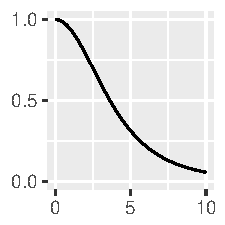
\includegraphics[width=1.5cm]{figs/compArel0}};}
\end{tikzpicture}
\end{frame}



%\nocite{2015:bayessurvsign}

\begin{frame}{References}
\renewcommand*{\bibfont}{\footnotesize}
%\begin{frame}[allowframebreaks]{References}
\printbibliography[heading=none,fontsize=\scriptsize]
\end{frame}

\end{document}
